% \documentclass{article}
% \usepackage[utf8]{inputenc}
% \usepackage{listings}
% \usepackage{xcolor}
% \usepackage{geometry}
% \usepackage{mathtools}
% \usepackage{listings}
% \usepackage{hyperref}
% \usepackage[ruled,vlined]{algorithm2e}
% \usepackage{float}
% \geometry{margin=1in}

% \begin{document}

\section{Algorithm}
Note that $X$ and $Y$ are the bipartitions of the bipartite graph $G$ and $M$ is some matching of $G$.

\vspace{0.5cm}

\begin{algorithm}[!h]
\caption{BFS}
\KwData{$X, Y, M$}
\KwResult{$G_{\mathrm{BFS}}$}

$G_{\mathrm{BFS}} \leftarrow$ empty graph

visited $\leftarrow$ empty Set

$Q \leftarrow$ empty Queue

\For{each node $v$ in $B_1$}{
    \If{$v \notin M$}{
        enqueue $v$ in $Q$

        add $v$ to visited
    }
}
\While{$Q$ is NOT empty}{

    $v \leftarrow$ dequeue from $Q$

    \uIf{$v \in X$}{
        \For{each edge $(v, w)$ adjacent to $v$ such that $(v, w) \notin M$}{
            add $(v, w)$ to $G_{\mathrm{BFS}}$
        
            \If{$w \in$ visited}{
                skip edge
            }
            enqueue $w$ in $Q$
        
            add $w$ to visited   
        }
    }\uElse{
        \For{each edge $(v, w)$ adjacent to $v$ such that $(v, w) \in M$}{
            add $(v, w)$ to $G_{\mathrm{BFS}}$
    
            \If{$w \in$ visited}{
                skip edge
            }
    
            enqueue $w$ in $Q$
    
            add $w$ to visited       
        }
    }
}

return $G_{\mathrm{BFS}}$
\end{algorithm}

\begin{algorithm}[!h]
\KwData{$G_{\mathrm{BFS}}, M, v$, visited, $P$}
\KwResult{Boolean}
\caption{ActualDFS}
\If{$v$ in visited}{return False}

add $v$ to visited

\For{all edges $(v, w)$ adjacent to $v$ in $G_{\mathrm{BFS}}$}{
    \If{($v \in X$ and $(v,w) \notin M$) or ($v \in Y$ and $(v,w) \in M$)}{skip edge}
    
    append $(v, w)$ to $P$
    
    \If{$w \notin M$}{
        add $w$ to visited
        return True
    }
    
    foundPath $\leftarrow$ actualDFS($G_{\mathrm{BFS}}, M, w$, visited, $P$)
    
    \If{foundPath is True}{return True}
    
    remove $(v, w)$ from $P$
}
return False
\end{algorithm}

\begin{algorithm}[!h]
\caption{DFS (wrapper)}
\KwData{$G_{\mathrm{BFS}}, M$}
\KwResult{set of disjoint paths}

visited $\leftarrow$ empty set

disjointPaths $\leftarrow$ empty set

\For{each node $v$ in $Y$}{
    \If{$v \notin M$}{
        $P \leftarrow$ empty path 

        ActualDFS($G_{\mathrm{BFS}}, M, v$, visited, $P$)

        add $P$ to disjointPaths if $P$ is NOT empty
    }
}
return disjointPaths
\end{algorithm}

\begin{algorithm}[!h]
\SetKwRepeat{Do}{do}{while}
\caption{HopcroftKarp}
\KwData{$X, Y, G$}
\KwResult{$M^*$}

$M \leftarrow$ empty matching

\Do{disjointPaths is NOT empty}{
    $G_{\mathrm{BFS}} \leftarrow$ BFS($X, Y, M$)

    disjointPaths $\leftarrow$ DFS($G_{\mathrm{BFS}}, M$)
    
    augment $M$ with each $P$ in disjointPaths
}
return $M$
\end{algorithm}


\section{Proof of Correctness}
\subsection{Augmenting Path Lemma}
Augmenting Path Lemma: A matching $M$ of $G$ is maximum if and only if there is no augmenting path in $G$.

This lemma has been proved in the lecture, so we use it as it is.

\subsection{Disjoint Paths Lemma}
Disjoint Path Lemma: The paths returned by the DFS subroutine are vertex disjoint and are augmenting paths of $M$ wrt $G$.

\begin{figure}[!h]
    \centering
    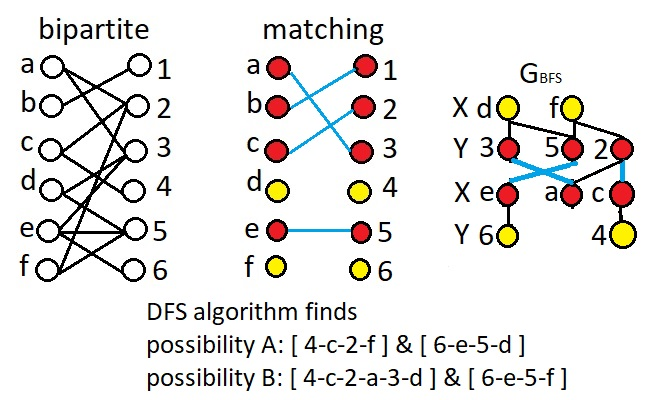
\includegraphics[scale=0.7]{hopcroftkarp_bfs.jpg}
    \caption{Finding Augmenting Paths}
\end{figure}

The graph formed by the BFS has 2 types of nodes, belonging to $X$ and belonging to $Y$. They can be imagined as stacks of layers going from top to bottom as shown in the figure. It is easy to see that the algorithm selects edges going from $X \to Y$ only when the edge is NOT present in the matching and selects edges going from $Y \to X$ only when the edge IS present in the matching.

Hence when we apply DFS from a node $v \in Y$, we are guaranteed to find a node $w \in X$ and $w \in M$ such that $(v, w) \notin M$. Similarly when we move from a node $v \in X $ and $v \in M$, we are guaranteed to find a node $w \in Y$ such that $(v, w) \in M$.

Also see that the DFS returns a path which begins and ends at nodes NOT present in the matching. Further the path contains edges alternate between $X$ and $Y$ such that all edges from $X \to Y \in M$ and all edges from $Y \to X \notin M$. Hence this path is an augmenting path.

Moreover this path is also disjoint since after using a node we immediately mark it as used. Hence it is effectively removed from the graph $G_{\mathrm{BFS}}$ and cannot be shared with any other path found by further iterations of the DFS algorithm.

\section{Time Complexity}

\subsection{Claim 1}
We make a claim that for a maximum matching $M^*$ and some matching matching $M$, the symmetric difference of $M^*$ and $M = M \Delta M^*$ has $|M^*|-|M|$ augmenting paths and these paths are vertex disjoint. 

We know that the presence of an augmenting path increases the size of $M$ by 1. So there are exactly $|M^*|-|M|$ augmenting paths. Also since the degree of each node is at max 2, the paths are vertex-disjoint.

\subsection{Claim 2}
We make a claim that there are at max $2\sqrt{N}$ iterations in the main loop. 

Notice that each iteration of the main algorithm increases the size of the matching by at least 1. Hence the shortest augmenting path is of length $\sqrt{N}$ after $\sqrt{N}$ iterations.

Since these paths will be vertex disjoint, we can say that there are at maximum $\sqrt{N}$ augmenting paths. Each of these paths increases the size of $M$ by 1 and hence $|M^*|-|M|$ is at max $\sqrt{N}$. Hence optimal matching $M^*$ will be achieved after at max $\sqrt{N}$ more iterations of the main algorithm.

\subsection{Calculating Time Complexity}
\begin{itemize}
    \item Each iteration involves BFS, DFS and augmenting $M$ with vertex disjoint paths.
    \item Both BFS and DFS take O$(|E|)$ time.
    \item Since the paths used to augment $M$ are vertex disjoint, the entire process takes O$(|V|)$ time.
    \item Hence each iteration of the main algorithm takes O$(|V|+|E|)$ = O($|E|$) time.
    \item From claim 2, we can see that there are at max O$(\sqrt{|V|})$ iterations.
\end{itemize}
So the overall time complexity is O($|E|\sqrt{|V|}$).

\section{Parallel Algorithm}
The main 2 components of the Hopcroft-Karp Algorithm are augmenting the matching and disjoint path finding in the bipartite graph. The augmentation of the matching is has a dependency i.e. to augment some matching, we need the matching itself. 

The second component i.e. disjoint path finding again consists of a modified BFS and DFS. Attempting the BFS in a prallel manner results in the need of synchronisation between the processors at such a high level that the parallelism is negligible even when ignoring overheads. Similarly is the case for DFS. To make the paths vertex disjoint we have to make use of mutual exclusion when considering the neighbours of a vertex. This again results in overheads (checking all neighbours of a vertex before performing the recursion) in the algorithm that actually increase the time complexity. 

However experiments have shown that using these techniques, an experimental speedup is obtained even with a poorer time complexity than the serial algorithm.

\section{Distributed Algorithm}
The algorithm can be distributed with the help of a central authority driving the phases of the algorithm performing the BFS in a synchronised manner (achieved with the help of the leader taking charge of this) and then a distributed alternating DFS while implementing look ahead strategy so that different vertices do not claim a single vertex to be part of two different augmenting paths since the paths needs to be vertex disjoint.

\section{References}
\begin{itemize}
    \item \href{https://en.wikipedia.org/wiki/Hopcroft\%E2\%80\%93Karp_algorithm}{\textcolor{blue}{Wikipedia article on the Hopcroft-Karp Algorithm}}
    \item \href{https://people.eecs.berkeley.edu/~aydin/matchingGraft.pdf}{\textcolor{blue}{A Parallel Tree Grafting Algorithm for Maximum Cardinality Matching in Bipartite Graphs by Ariful Azad, Aydin Buluc, Alex Pothen}}
    \item \href{https://link.springer.com/article/10.1007\%2FBF01840395}{\textcolor{blue}{Michael M. Wu; Michael C. Loui (1990). An efficient distributed algorithm for maximum matching in general graphs}}
\end{itemize}




%\end{document}
